\section{Результаты}
В эксперименте использована установка, состоящая из двух резервуаров. Сосуды соединены трубкой, оснащенной краном $K_3$, через которую диффундирующий газ перетекает из одного сосуда в другой. Сосуды подключены к системе напуска и откачки гелия и воздуха (краны $K_1$ и $K_2$ позволяют накачивать газы по отдельности в каждый сосуд). Также к системе подключен манометр. Важная особенность установки, позволяющая использовать формулу \eqref{eq:delta_n_t}, верную только для квазистационарного потока газа, заключается в том, что объем трубки, соединяющей два резервуара, много меньше объемов сосудов ($LS\ll V$).

Более подробное описание установки см. в \nameref{Приложение}.

Параметры установки:
\begin{center}
    $V= (775 \pm 10)\text{см}^3$
    
    $\frac{L}{S} = (5.3 \pm 0.1)\frac{1}{\text{см}}$

   
\end{center}
 $L$ - длина трубки, в которой происходит диффузия,

 $S$ - площадь поперечного сечения этой трубки
 (в приложение)
Перед каждым измерением искомой зависимости, описанной в методике, установка была подготовлена: в сосуды была закачана смесь гелия и воздуха до определенного давления. Давление измерялось с помощью манометра, подключенного к соединительным трубкам. Он показывает разность давлений между соединительными трубками и атмосферой и позволяет измерять давления в разных частях системы (в зависимости от положения кранов).

Разность напряжений на нагревательных элементах - проволоках ($\text{Д}_1, \text{Д}_2$), расположенных в сосудах, измерялась с помощью мостовой схемы (см. \nameref{Приложение}).


Перед каждым измерением установка была подключена к насосу и откачана до давления $\sim 0.1$ торр. Затем в установку напускался воздух до рабочего давления в диапазоне от 40 до 300 торр, и производилась балансировка моста (при запертых кранах $K_1, K_2$, $K_3$ - открыт). Затем установка снова откачивалась до давления $\sim 0.1$ торр. При изолированном объеме $V_2$, в установку был закачан гелий до давления $P_{He} = 0.2P$ (кран $K_7$ открыт), для более точной накачки был использован дозатор. Теперь, когда один из сосудов ($V_1$) заполнен гелием, в объем $V_2$ был напущен воздух до давления $P_{возд}=1.675P$ при изолированном объеме $V_1$. Затем были уравнены давления в сосудах путем открытия кранов $K_1$ и $K_2$ при закрытых $K_3$ и $K_4$. Поскольку газ при адиабатическом расширении остывает, краны $K_1$ и $K_2$ были открытыми в течение 30-60 с., чтобы дать давлениям выравняться при одинаковых температурах. Это время не должно быть слишком велико, чтобы диффузия гелия по патрубкам в обратном направлении не привела к искажению приготовленного состояния.

По измеренным зависимостям $U(t)$ для 6 различных рабочих давлений с помощью компьютерной программы, построены линеаризованные графики.
Результаты измерения разности концентраций от времени представлены на рисунке
\begin{center}
    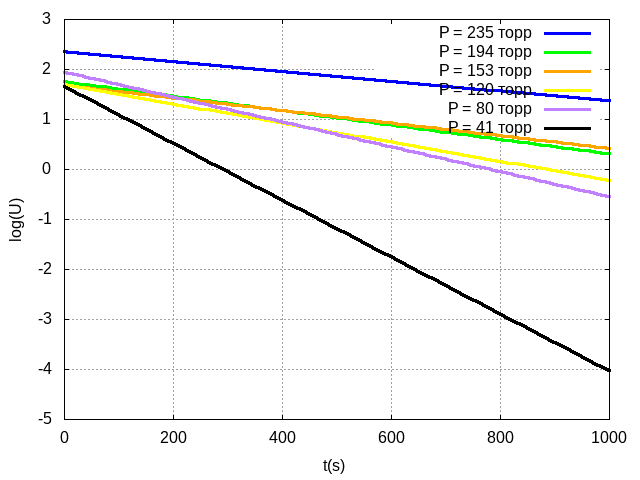
\includegraphics[width=0.9\textwidth]{img/graph1.png}
    
    Графики зависимости $ln(U)(t)$
\end{center}

График, изображенный на рисунке, является линейным, следовательно, эксперимент согласуется с теорией и разность ($\Delta n$) концентраций связана со временем ($t$) выражением \eqref{eq:delta_n_t}.

По методу наименьших квадратов определены коэффициенты наклона прямых, которые по значениям совпадают с коэффициентом $-\frac{1}{\tau}$ из выражения \eqref{eq: ln(U)_t}.
\begin{equation}
    k = -\frac{1}{\tau} \propto D \label{eq: k}
\end{equation}
\begin{center}
    $k_{41} = (-0.00569 \pm 0.00021)\text{с}^{-1}$
    
    $k_{80} = (-0.00249 \pm 0.00005)\text{с}^{-1}$
    
    $k_{120} = (-0.00191 \pm 0.00004)\text{с}^{-1}$
    
    $k_{153} = (-0.001262 \pm 0.000020)\text{с}^{-1}$
    
    $k_{194} = (-0.001440 \pm 0.000020)\text{с}^{-1}$
    
    $k_{235} = (-0.000980 \pm 0.000009)\text{с}^{-1}$

    $\epsilon_{41} = 3.622\%$

    $\epsilon_{80} = 1.865\%$

    $\epsilon_{120} = 1.895\%$

    $\epsilon_{153} = 1.552\%$

    $\epsilon_{194} = 1.411\%$

    $\epsilon_{235} = 0.8693\%$
\end{center}



Из графика и выражения \eqref{eq: k} следует, что с увеличением давления уменьшается коэффициент диффузии. Коэффициент диффузии линейно выражается через длину свободного пробега молекул газа
\begin{equation}
    D = \frac{1}{3} \lambda v \label{eq: D}
\end{equation}
где $\lambda$ - длина свободного пробега молекулы, 
$\lambda = \frac{1}{\sigma n}$,
$n$ - концентрация молекулярного фона.
При увеличении давления увеличивается концентрация молекул, следовательно, уменьшается длина свободного пробега (молекулы чаще ударяются друг о друга). Так как $D \propto \lambda$, то коэффициент диффузии уменьшается.

Рассчитанные значения $\tau$ для каждого давления представлены в таблице (см. \nameref{Приложение}).

Рассчитанные значения $D$ для каждого давления представлены в таблице (см. \nameref{Приложение})

Используя данные из таблицы (см. \nameref{Приложение}), построили график зависимости $D(\frac{1}{P})$

\begin{center}
    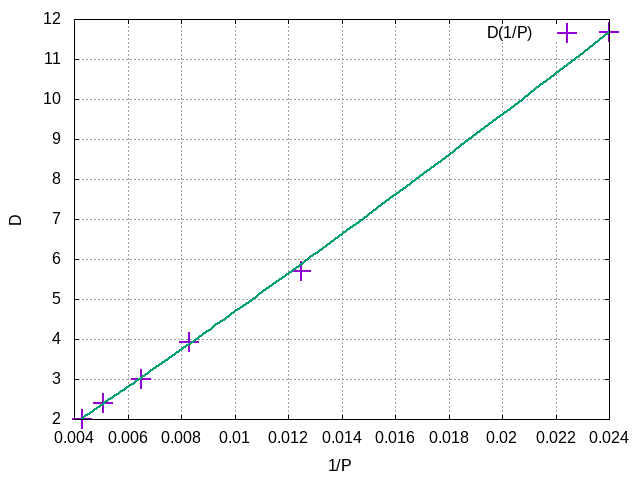
\includegraphics[width=0.9\textwidth]{img/graph3 (1).png}
    
    График зависимости $D(\frac{1}{P})$
\end{center}

Из графика видно, что $D$ линейно зависит от $\frac{1}{P}$, что удовлетворяет предположению теории.  В общем случае, при учете диффузии каждого из компонентов смеси (в работе рассматривалась диффузия легких и подвижных молекул гелия на фоне тяжелых и неподвижных молекул воздуха) выражение \eqref{eq: D} сохраняется, если под $\lambda$ понимать величину $\lambda = \frac{1}{n_{\sum}\sigma}$, где $n_{\sum} = n_{He}+n_{\text{возд}} = \frac{P}{k_\text{Б}T}$ - полная концентрация частиц смеси и под $v$ понимать среднюю относительную скорость частиц разных сортов. Таким образом 
    \begin{equation}
        D = \frac{1}{3}\lambda v = \frac{1}{3}\frac{k_{\text{Б}}T}{P\sigma} \propto \frac{1}{P}
    \end{equation}

С помощью метода наименьших квадратов определили значение углового коэффициента 
$k = (479.15 \pm 33.63)\frac{\text{см}^2}{c\cdot \text{торр}}$ и свободного члена $b = (-0.1407 \pm 0.4091)\frac{\text{см}^2}{c}$

По графику определили коэффициент диффузии при атмосферном давлении:
\begin{equation}
     D_{\text{атм}} = k \cdot \frac{1}{P_\text{атм}} + b
\end{equation}

\[ D_{\text{атм}} = (0.49 \pm 0.03)\frac{\text{см}^2}{c}\]

(Оценка времени распространения радиоактивного облака)

